%%%%%%%%%%%%%%%%%%%%%%%%%%%%%%%%%%%%%%%%%%%%%%
% An example of a lab report write-up.
%%%%%%%%%%%%%%%%%%%%%%%%%%%%%%%%%%%%%%%%%%%%%%
% This is a combination of several labs that I have done in the past for
% Computer Engineering, so it is not to be taken literally, but instead used as
% a great starting template for your own lab write up.  When creating this
% template, I tried to keep in mind all of the functions and functionality of
% LaTeX that I spent a lot of time researching and using in my lab reports and
% include them here so that it is fairly easy for students first learning LaTeX
% to jump on in and get immediate results.  However, I do assume that the
% person using this guide has already created at least a "Hello World" PDF
% document using LaTeX (which means it's installed and ready to go).
%
% My preference for developing in LaTeX is to use the LaTeX Plugin for gedit in
% Linux.  There are others for Mac and Windows as well (particularly MikTeX).
% Another excellent plugin is the Calc2LaTeX plugin for the OpenOffice suite.
% It makes it very easy to create a large table very quickly.
%
% Professors have different tastes for how they want the lab write-ups done, so
% check with the section layout for your class and create a template file for
% each class (my recommendation).
%
% Also, there is a list of common commands at the bottom of this document.  Use
% these as a quick reference.  If you'd like more, you can view the "LaTeX Cheat
% Sheet.pdf" included with this template material.
%
% (c) 2009 Derek R. Hildreth <derek@derekhildreth.com> http://www.derekhildreth.com
% This work is licensed under the Creative Commons Attribution-NonCommercial-ShareAlike License. To view a copy of this license, visit http://creativecommons.org/licenses/by-nc-sa/1.0/ or send a letter to Creative Commons, 559 Nathan Abbott Way, Stanford, California 94305, USA.
%%%%%%%%%%%%%%%%%%%%%%%%%%%%%%%%%%%%%%%%%%%%%%
\documentclass[aps,letterpaper,10pt]{revtex4}
\input kvmacros % For Karnaugh Maps (K-Maps)

\usepackage{graphicx} % For images
\usepackage{float}    % For tables and other floats
\usepackage{verbatim} % For comments and other
\usepackage{amsmath}  % For math
\usepackage{amssymb}  % For more math
\usepackage{fullpage} % Set margins and place page numbers at bottom center
\usepackage{listings} % For source code
\usepackage{subfig}   % For subfigures
\usepackage[usenames,dvipsnames]{color} % For colors and names
\usepackage{hyperref}           % For hyperlinks and indexing the PDF
\usepackage{listings}
\usepackage{color}

\definecolor{dkgreen}{rgb}{0,0.6,0}
\definecolor{gray}{rgb}{0.5,0.5,0.5}
\definecolor{mauve}{rgb}{0.58,0,0.82}

\lstset{frame=tb,
  language=Python,
  aboveskip=3mm,
  belowskip=3mm,
  showstringspaces=false,
  columns=flexible,
  basicstyle={\small\ttfamily},
  numbers=none,
  numberstyle=\tiny\color{gray},
  keywordstyle=\color{blue},
  commentstyle=\color{dkgreen},
  stringstyle=\color{mauve},
  breaklines=true,
  breakatwhitespace=true,
  tabsize=3
}
%==========================================================================
\hypersetup{ % play with the different link colors here
    colorlinks,
    citecolor=blue,
    filecolor=blue,
    linkcolor=blue,
    urlcolor=blue % set to black to prevent printing blue links
}

\definecolor{mygrey}{gray}{.96} % Light Grey
\lstset{
	language=[ISO]C++,              % choose the language of the code ("language=Verilog" is popular as well)
   tabsize=3,							  % sets the size of the tabs in spaces (1 Tab is replaced with 3 spaces)
	basicstyle=\tiny,               % the size of the fonts that are used for the code
	numbers=left,                   % where to put the line-numbers
	numberstyle=\tiny,              % the size of the fonts that are used for the line-numbers
	stepnumber=2,                   % the step between two line-numbers. If it's 1 each line will be numbered
	numbersep=5pt,                  % how far the line-numbers are from the code
	backgroundcolor=\color{mygrey}, % choose the background color. You must add \usepackage{color}
	%showspaces=false,              % show spaces adding particular underscores
	%showstringspaces=false,        % underline spaces within strings
	%showtabs=false,                % show tabs within strings adding particular underscores
	frame=single,	                 % adds a frame around the code
	tabsize=3,	                    % sets default tabsize to 2 spaces
	captionpos=b,                   % sets the caption-position to bottom
	breaklines=true,                % sets automatic line breaking
	breakatwhitespace=false,        % sets if automatic breaks should only happen at whitespace
	%escapeinside={\%*}{*)},        % if you want to add a comment within your code
	commentstyle=\color{BrickRed}   % sets the comment style
}

% Make units a little nicer looking and faster to type
\newcommand{\Hz}{\textsl{Hz}}
\newcommand{\KHz}{\textsl{KHz}}
\newcommand{\MHz}{\textsl{MHz}}
\newcommand{\GHz}{\textsl{GHz}}
\newcommand{\ns}{\textsl{ns}}
\newcommand{\ms}{\textsl{ms}}
\newcommand{\s}{\textsl{s}}



% TITLE PAGE CONTENT %%%%%%%%%%%%%%%%%%%%%%%%
% Remember to fill this section out for each
% lab write-up.
%%%%%%%%%%%%%%%%%%%%%%%%%%%%%%%%%%%%%%%%%%%%%
\newcommand{\labno}{05}
\newcommand{\labtitle}{AU 332 Artificial Intelligence: Principles and Techniques}
\newcommand{\authorname}{Chi Zhang (517021910658)}
\newcommand{\hw}{0}
% END TITLE PAGE CONTENT %%%%%%%%%%%%%%%%%%%%


\begin{document}  % START THE DOCUMENT!


% TITLE PAGE %%%%%%%%%%%%%%%%%%%%%%%%%%%%%%%%%%%%%%
% If you'd like to change the content of this,
% do it in the "TITLE PAGE CONTENT" directly above
% this message
%%%%%%%%%%%%%%%%%%%%%%%%%%%%%%%%%%%%%%%%%%%%%%%%%%%
\begin{titlepage}
\begin{center}
{\Large \textsc{\labtitle} \\ \vspace{4pt}}
\rule[13pt]{\textwidth}{1pt} \\ \vspace{150pt}
{\large By: \authorname \\ \vspace{10pt}
HW\#: \hw \\ \vspace{10pt}
\today}
\end{center}
\end{titlepage}
% END TITLE PAGE %%%%%%%%%%%%%%%%%%%%%%%%%%%%%%%%%%





%%%%%%%%%%%%%%%%%%%%%%%%%%%%%%
%%%%%%%%%%%%%%%%%%%%%%%%%%%%%%
\section{Introduction}
%No Text Here
%%%%%%%%%%%%%%%%%%%%%%%%%%%%%%%
\subsection{Purpose}
\begin{comment}
This is a lab template which has a ton of different things which are useful in writing lab write-ups in the Computer Eningeering field.  This is demonstrating the comment block. Don't be overwhelmed, it may seem like a lot to take in at a time, but it's worth spending the time learning it.
\end{comment}
As required by Question 1, 2 and 3, my function need to implement following features :
\begin{itemize}
	\item Question 1: Enter a and b, and return the sum of a and b
	\item Question 2: Enter a list of \texttt{(fruit, pound)} tuples and return the cost of the fruit in the list. 
	If the list contains some fruit that not in the \texttt{fruitPrices}, the funtion will print an error message and return \textbf{None}
	\item Question 3: Enter a list of \texttt{(fruit, pound)} tuples and a list of \texttt{fruitshop}, 
	and return the shop which the account is least. 
\end{itemize}

\vspace{3mm} % I use this to seperate the paragraphs a bit.

The homework aims to help us familiar with Python, especially the usage of function and class.

%%%%%%%%%%%%%%%%%%%%%%%%%%%%%%
\subsection{Equipment}
There is a minimal amount of equipment to be used in this lab.  The few requirements are listed below:
	\begin{itemize}
		\item Python 3.7.0 (Anaconda)
	\end{itemize}

%%%%%%%%%%%%%%%%%%%%%%%%%%%%%%
\subsection{Procedure}
\subsubsection{Problem 1}
The function of Problem 1 is simple, I just return \texttt{(a+b)} .
\begin{lstlisting}
	def add(a, b):
    "print the sum of a and b"
    "*** YOUR CODE HERE ***"
    return (a+b)
\end{lstlisting}

\subsubsection{Problem 2}
The function \textbf{buyLotsOfFruit} receive a list of (fruit, numPounds) tuples, which means we can use the \emph{for} statement
to read all the fruit and weight in the list

In my code, I use \texttt{fruit} to represent the element in the list, therefore, fruit[0] is the variety of fruit and fruit[0] is the weight of this fruit.
Before I compute the cost of each kind of fruit, I use the \emph{if} statement to judge if this fruit is in the \texttt{fruitPrices}. If not, the function will print an error message and the function will return \textbf{None} as result.


\begin{lstlisting}
	def buyLotsOfFruit(orderList):
    """
        orderList: List of (fruit, numPounds) tuples

    Returns cost of order
    """
    totalCost = 0.0
    "*** YOUR CODE HERE ***"
    for fruit in orderList:
        if fruit[0] in fruitPrices:
            totalCost += fruitPrices[fruit[0]] * fruit[1]
        else :
            totalCost = None
            print('error! '+fruit[0]+ ' is not in the fruitPrices list')
            break

    return totalCost
\end{lstlisting}

\subsubsection{Problem 3}

The file \texttt{shop.py} has defined class \texttt{FruitShop}, which includes function \texttt{getCostPerPound} and \texttt{getPriceOfOrder}. In my 
code, I use \texttt{the\underline{ }shop} to represent the shop in the \texttt{fruitShops} list. In each loop, \texttt{the\underline{ }shop.getPriceOfOrder} will compute 
the cost of the order in current shop. Besides, I create variable \texttt{least\underline{ }amount} and \texttt{correspond\underline{ }shop} to record the lowest cost and corresponding name of shop.


\begin{lstlisting}
	def shopSmart(orderList, fruitShops):
    """
        orderList: List of (fruit, numPound) tuples
        fruitShops: List of FruitShops
    """
    "*** YOUR CODE HERE ***"
    least_amount = None
    correspond_shop = None
    for the_shop in fruitShops:
        current_amount = the_shop.getPriceOfOrder(orderList)
        if least_amount is None or least_amount > current_amount :
            least_amount = current_amount
            correspond_shop = the_shop

    return correspond_shop
\end{lstlisting}

%%%%%%%%%%%%%%%%%%%%%%%%%%%%%%
%%%%%%%%%%%%%%%%%%%%%%%%%%%%%%
\newpage
\section{Experiment}
This section consists of screenshots taken during the laboratory procedure. 

	% You can refer to this set of images by using \ref{fig:oscil}.  ie "please refer to Figure \ref{fig:oscil}."
	% You can refer to a specific subimage by using \ref{fig:Per6A}. ie "please refer to Figure \ref{fig:Per6A}."
   % I prefer the quality of a .png image, but you may use other extensions such as .jpg.
	\begin{figure}[H]
	  \centering
	  \subfloat[test code for \texttt{add}]{\label{fig:Per6A}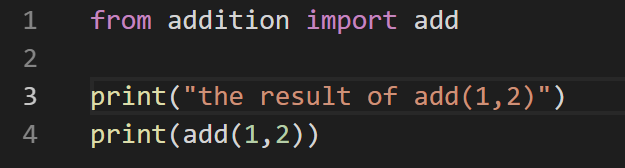
\includegraphics[width=0.4\textwidth]{add_code.png}} \\
	  \subfloat[result of the test]{\label{fig:Per6A}
\includegraphics[width=0.4\textwidth]{add_result.png}}
	  \caption{Figures of the test for question 1}
	  \label{fig:oscil}
	\end{figure}

	\begin{figure}[H]
		\centering
		\subfloat[test code for \texttt{buyLotsOfFruit}]{\label{fig:Per6A}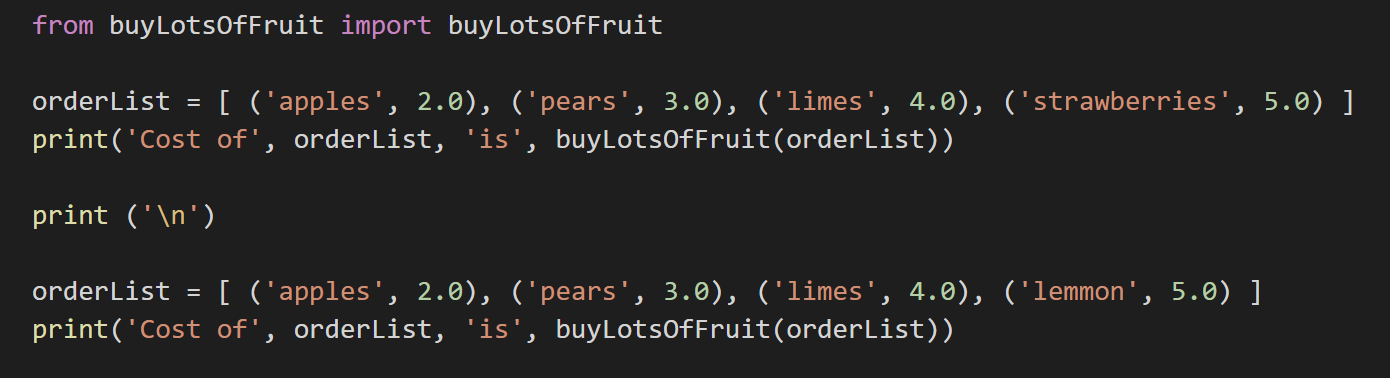
\includegraphics[width=0.8\textwidth]{cost_code.png}} \\
		\subfloat[result of the test]{\label{fig:Per6A}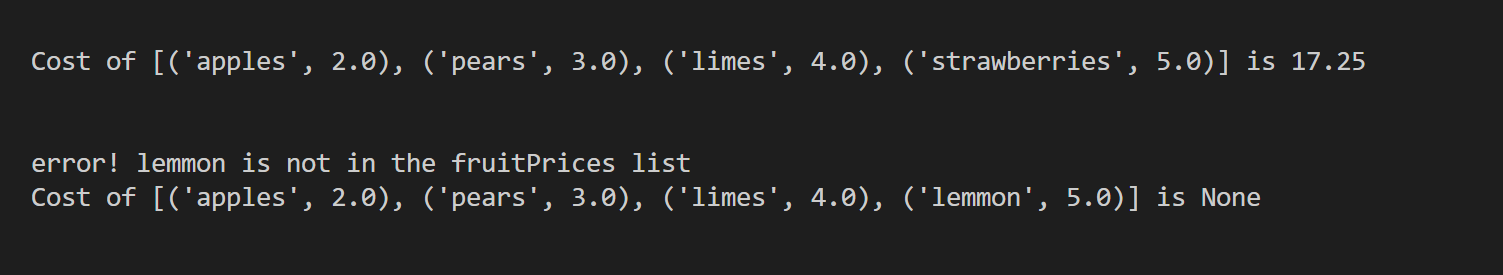
\includegraphics[width=0.8\textwidth]{cost_result.png}}
		\caption{Figures of the test for question 2}
		\label{fig:oscil}
	\end{figure}

	\begin{figure}[H]
		\centering
		\subfloat[test code for \texttt{shopSmart}]{\label{fig:Per6A}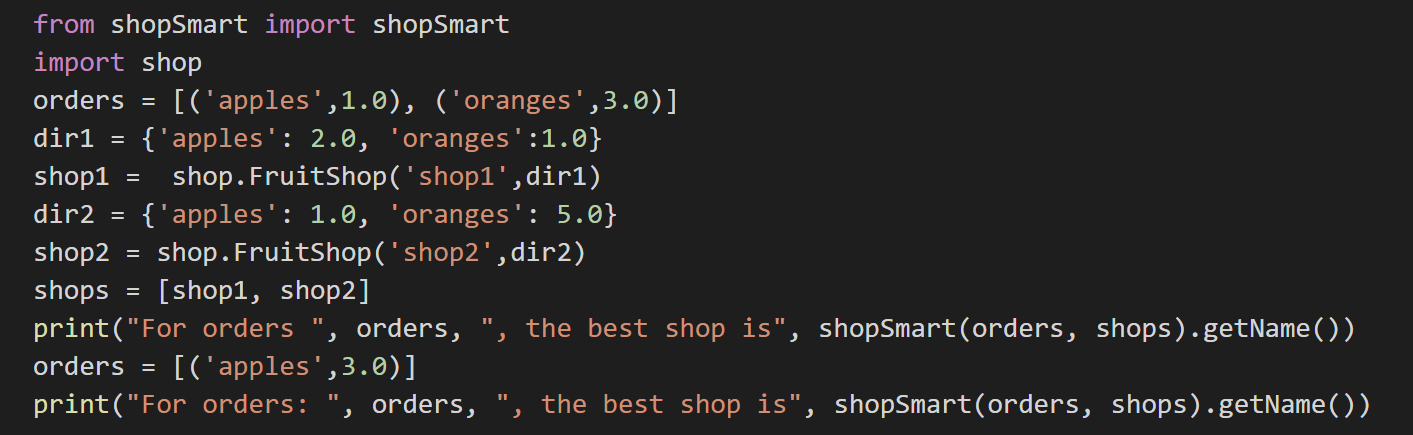
\includegraphics[width=0.8\textwidth]{shop_code.png}} \\
		\subfloat[result of the test]{\label{fig:Per6A}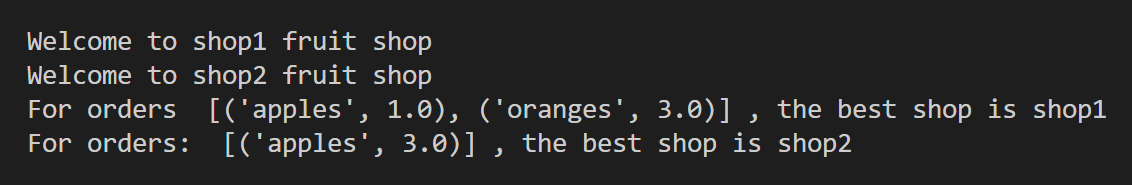
\includegraphics[width=0.8\textwidth]{shop_result.png}}
		\caption{Figures of the test for question 3}
		\label{fig:oscil}
	\end{figure}

%%%%%%%%%%%%%%%%%%%%%%%%%%%%%%
%%%%%%%%%%%%%%%%%%%%%%%%%%%%%%
\newpage


\section{Discussion \& Conclusion}
The homework is not difficult. It is aimed to help students get accustomed to \emph{Python}, and learn how to write reports with \emph{Latex}. I am unfamiliar with the usage of \emph{class} in \emph{Python}, 
and I know little about \emph{Latex}, so I spent lots of time on this homework.

\end{document} % DONE WITH DOCUMENT!


%%%%%%%%%%
PERSONAL FAVORITE LAB WRITE-UP STRUCTURE
%%%%%%%%%%
\section{Introduction}
	% No Text Here
	\subsection{Purpose}
		% Lab objective
	\subsection{Equipment}
		% Any and all equipment used (specific!)
	\subsection{Procedure}
		% Overview of the procedure taken (not-so-specific!)
\newpage
\section{Schematic Diagrams}
	% Any schematics, screenshots, block
   % diagrams used.  Possibly photos or
	% images could go here as well.
\newpage
\section{Experiment Data}
	% Depending on lab, program code would be
	% included here without the Estimated and
	% Actual Results.
	\subsection{Estimated Results}
		% Calculated. What it should be.
	\subsection{Actual Results}
		% Measured.  What it actually was.
\newpage
\section{Discussion \& Conclusion}
	% 3 Paragraphs:
		% Restate the objective of the lab
		% Discuss personal trials, errors, and difficulties
		% Conclude the lab


%%%%%%%%%%%%%%%%
COMMON COMMANDS:
%%%%%%%%%%%%%%%%
% IMAGES
begin{figure}[H]
   \begin{center}
      \includegraphics[width=0.6\textwidth]{RTL_SCHEM.png}
   \end{center}
\caption{A screenshot of the RTL Schematics produced from the Verilog code.}
\label{RTL}
\end{figure}

% SUBFIGURES IMAGES
\begin{figure}[H]
  \centering
  \subfloat[LED4 Period]{\label{fig:Per4}\includegraphics[width=0.4\textwidth]{period_led4.png}} \\
  \subfloat[LED5 Period]{\label{fig:Per5}\includegraphics[width=0.4\textwidth]{period_led5.png}}
  \subfloat[LED6 Period]{\label{fig:Per6}\includegraphics[width=0.4\textwidth]{period_led6.png}}
  \caption{Period of LED blink rate captured by osciliscope.}
  \label{fig:oscil}
\end{figure}

% INSERT SOURCE CODE
\lstset{language=Verilog, tabsize=3, backgroundcolor=\color{mygrey}, basicstyle=\small, commentstyle=\color{BrickRed}}
\lstinputlisting{MODULE.v}

% TEXT TABLE
\begin{table}
\begin{center}
\begin{tabular}{|l|c|c|l|}
	x & x & x & x \\ \hline
	x & x & x & x \\
	x & x & x & x \\ \hline
\end{tabular}
\caption{Caption}
\label{label}
\end{center}
\end{table}

% MATHMATICAL ENVIRONMENT
$ 8 = 2 \times 4 $

% CENTERED FORMULA
\[  \]

% NUMBERED EQUATION
\begin{equation}
	
\end{equation}

% ARRAY OF EQUATIONS (The splat supresses the numbering)
\begin{align*}
	
\end{align*}

% NUMBERED ARRAY OF EQUATIONS
\begin{align}
	
\end{align}

% ACCENTS
\dot{x} % dot
\ddot{x} % double dot
\bar{x} % bar
\tilde{x} % tilde
\vec{x} % vector
\hat{x} % hat
\acute{x} % acute
\grave{x} % grave
\breve{x} % breve
\check{x} % dot (cowboy hat)

% FONTS
\mathrm{text} % roman
\mathsf{text} % sans serif
\mathtt{text} % Typewriter
\mathbb{text} % Blackboard bold
\mathcal{text} % Caligraphy
\mathfrak{text} % Fraktur

\textbf{text} % bold
\textit{text} % italic
\textsl{text} % slanted
\textsc{text} % small caps
\texttt{text} % typewriter
\underline{text} % underline
\emph{text} % emphasized

\begin{tiny}text\end{tiny} % Tiny
\begin{scriptsize}text\end{scriptsize} % Script Size
\begin{footnotesize}text\end{footnotesize} % Footnote Size
\begin{small}text\end{small} % Small
\begin{normalsize}text\end{normalsize} % Normal Size
\begin{large}text\end{large} % Large
\begin{Large}text\end{Large} % Larger
\begin{LARGE}text\end{LARGE} % Very Large
\begin{huge}text\end{huge}   % Huge
\begin{Huge}text\end{Huge}   % Very Huge


% GENERATE TABLE OF CONTENTS AND/OR TABLE OF FIGURES
% These seem to have some issues with the "revtex4" document class.  To use, change
% the very first line of this document to "article" like this:
% \documentclass[aps,letterpaper,10pt]{article}
\tableofcontents
\listoffigures
\listoftables

% INCLUDE A HYPERLINK OR URL
\url{http://www.derekhildreth.com}
\href{http://www.derekhildreth.com}{Derek Hildreth's Website}

% FOR MORE, REFER TO THE "LINUX CHEAT SHEET.PDF" FILE INCLUDED!
